%
% $LastChangedRevision: 1896 $
% $LastChangedDate:: 2020-04-29 15:30:11 +0200#$
%
% This file is part of X2C. http://x2c.lcm.at/
%
% Copyright (c) 2013, Linz Center of Mechatronics GmbH (LCM) http://www.lcm.at/
% All rights reserved.
%
%
% This file is licensed according to the BSD 3-clause license as follows:
%
% Redistribution and use in source and binary forms, with or without
% modification, are permitted provided that the following conditions are met:
%     * Redistributions of source code must retain the above copyright
%       notice, this list of conditions and the following disclaimer.
%     * Redistributions in binary form must reproduce the above copyright
%       notice, this list of conditions and the following disclaimer in the
%       documentation and/or other materials provided with the distribution.
%     * Neither the name of the "Linz Center of Mechatronics GmbH" and "LCM" nor
%       the names of its contributors may be used to endorse or promote products
%       derived from this software without specific prior written permission.
%
% THIS SOFTWARE IS PROVIDED BY THE COPYRIGHT HOLDERS AND CONTRIBUTORS "AS IS" AND
% ANY EXPRESS OR IMPLIED WARRANTIES, INCLUDING, BUT NOT LIMITED TO, THE IMPLIED
% WARRANTIES OF MERCHANTABILITY AND FITNESS FOR A PARTICULAR PURPOSE ARE DISCLAIMED.
% IN NO EVENT SHALL "Linz Center of Mechatronics GmbH" BE LIABLE FOR ANY
% DIRECT, INDIRECT, INCIDENTAL, SPECIAL, EXEMPLARY, OR CONSEQUENTIAL DAMAGES
% (INCLUDING, BUT NOT LIMITED TO, PROCUREMENT OF SUBSTITUTE GOODS OR SERVICES;
% LOSS OF USE, DATA, OR PROFITS; OR BUSINESS INTERRUPTION) HOWEVER CAUSED AND
% ON ANY THEORY OF LIABILITY, WHETHER IN CONTRACT, STRICT LIABILITY, OR TORT
% (INCLUDING NEGLIGENCE OR OTHERWISE) ARISING IN ANY WAY OUT OF THE USE OF THIS
% SOFTWARE, EVEN IF ADVISED OF THE POSSIBILITY OF SUCH DAMAGE.
%
\XtoCBlock{Outport}
\label{block:Outport}
\begin{figure}[H]
\includegraphics{Outport}\end{figure} 

\begin{XtoCtabular}{Outports}
OUT & Signal to frame program\tabularnewline
\hline
\end{XtoCtabular}


\begin{XtoCtabular}{Mask Parameters}
ts\_fact & Multiplication factor of base sampling time (in integer format)\tabularnewline
\hline
Gain & Gain value used in simulation\tabularnewline
\hline
Offset & Offset value used in simulation\tabularnewline
\hline
\end{XtoCtabular}

\subsubsection*{Description:}
Serves as interface to the frame program. The output of this block is intended for simulation purposes and can be left unconnected if not used. Also the parameters \textit{Gain}, and \textit{Offset} are only used during simulation. The schematic for simulation can be seen in the figure below. The Unit Delay block is only used during simulation and should reflect the time delay caused by a discrete controller.

\textbf{Note:} Currently, \textit{Gain} and \textit{Offset} parameters are only available in Matlab/Simulink.
\begin{figure}[H]
  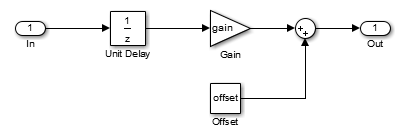
\includegraphics{Outport_Schematic}
\end{figure}

\subsubsection*{Data Types:}
\begin{tabular}{l l}
\textbf{int8} & 8 Bit Fixed Point\tabularnewline
\textbf{int16} & 16 Bit Fixed Point\tabularnewline
\textbf{int32} & 32 Bit Fixed Point\tabularnewline
\textbf{float32} & 32 Bit Floating Point\tabularnewline
\textbf{float64} & 64 Bit Floating Point\tabularnewline
\end{tabular}
